\begin{frame}{Japanese vs. Chinese}
	\begin{center}
		\begin{CJK*}{UTF8}{gkai}
		\Huge 电
		\end{CJK*}
	\\
	\onslide<2>{Chinese}
	\end{center}
\end{frame}

\begin{frame}{Training / Fitting}
	\begin{center}
		\huge \textbf{Japanese} {\small (hiragana)}\\
		\begin{CJK*}{UTF8}{min}
			\Huge ま ち ね ら に ご
		\end{CJK*}
		\\
		\vspace{2em}

		\huge \textbf{Chinese} {\small (kanji)}\\
		\begin{CJK*}{UTF8}{gkai}
			\Huge 电 买 开 东 车 红 马
		\end{CJK*}
	\end{center}
\end{frame}

\begin{frame}{Application / Inference}
	\begin{center}
		\begin{CJK*}{UTF8}{min}
			\Huge の
		\end{CJK*}
		\\
		\onslide<2>{Japanese\\}
		\vspace*{1em}
		\begin{CJK*}{UTF8}{min}
			\Huge る
		\end{CJK*}
		\\
		\onslide<3>{Japanese\\}
		\vspace*{1em}
		\begin{CJK*}{UTF8}{gkai}
			\Huge 热
		\end{CJK*}
	    \\
		\onslide<4>{Chinese\\}
		 \vspace*{1em}
		\begin{CJK*}{UTF8}{gkai}
			\Huge 时
		\end{CJK*}
		\\
		\onslide<5>{Chinese\\}
		 \vspace*{1em}
		\begin{CJK*}{UTF8}{min}
			\Huge な
		\end{CJK*}
		\\
		\onslide<6>{Japanese}

	\end{center}
\end{frame}

\begin{frame}
	\begin{center}
		{\huge \textbf{Congratulation!}} \\
         {\large You are an intelligent entity} \\
         \vspace*{3em}
         
         \onslide<2>{\large \textcolor{Treddark}{Let's build a machine that can do this!}}
	\end{center}
\end{frame}


\begin{frame}{Machine Learning}
	\begin{center}
		\hspace{0.5em}\includegraphics[width=0.45\textwidth]{go.jpg}\hspace{0.5em}
		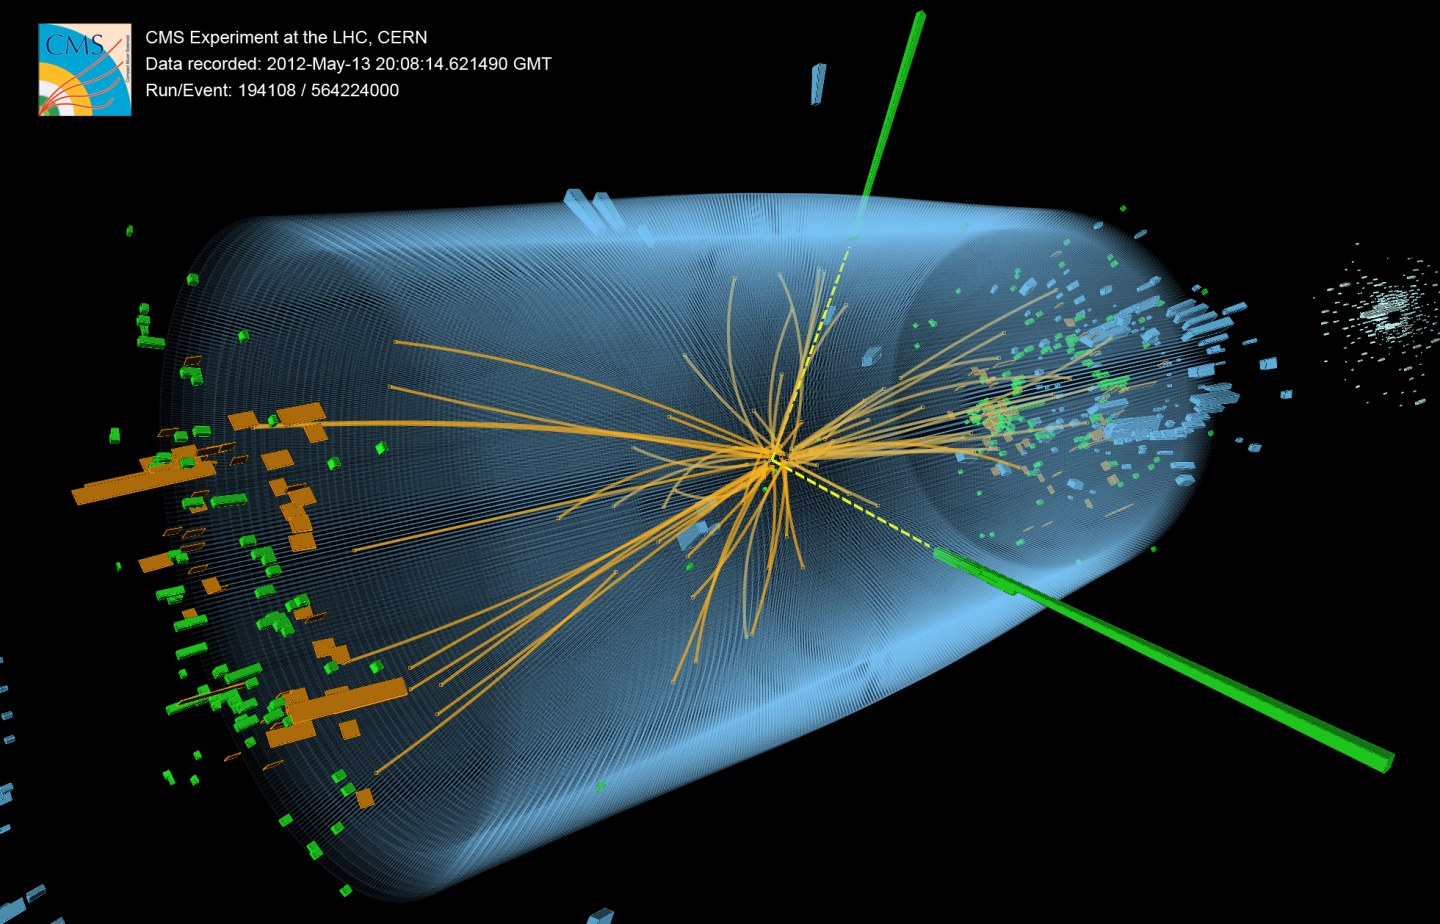
\includegraphics[width=0.45\textwidth]{higgs.png}\\
		\vspace*{0.5em}
		\hspace{0.5em}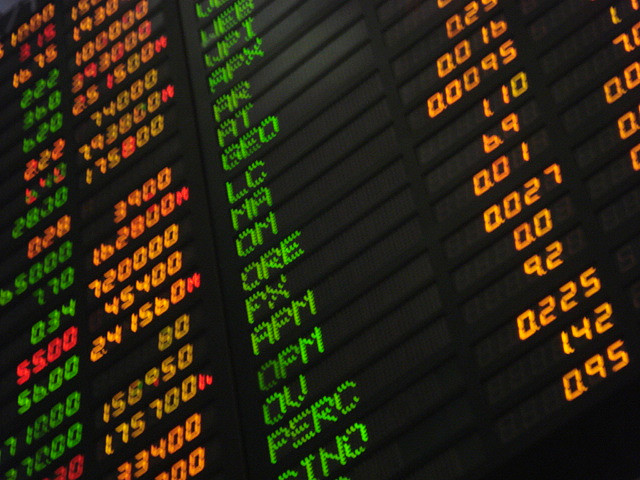
\includegraphics[width=0.45\textwidth]{stock.jpg}\hspace{0.5em}
		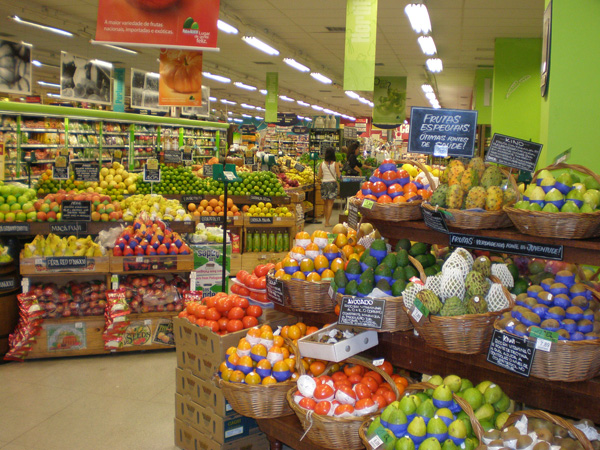
\includegraphics[width=0.45\textwidth]{supermarkt.jpg}\\
	\end{center}
\end{frame}

{
	\usebackgroundtemplate{  
		\tikz { 
			\fill[white] (0,0) rectangle (16,-2);
			\fill[Tredlight!20] (0,-2) rectangle (16,-4.3);
		    \fill[Tyellowlight!20] (0,-4.3) rectangle (16,-7.7);
		    \fill[Tgreenlight!20] (0,-7.7) rectangle (16,-10);
		}
	}
\begin{frame}{Machine Learning}

		\begin{columns}[t]
			\begin{column}{0.3\textwidth}
					\begin{center}
						\vspace{-1em}
        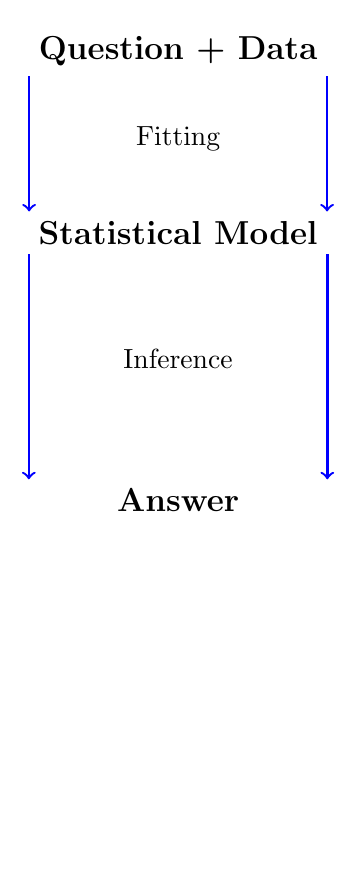
\begin{tikzpicture}
        \node (x) at (0, 2) {};
        \node (x) at (0, -7) {};
        \node (data) at (0,3) {\large \textbf{Question + Data}};

		\node (model) at (0,0.7) {\large \textbf{Statistical Model}};

		\node (answer) at (0,-2.7) {\large \textbf{Answer}};

		\onslide<4->{
				\node (fitting) at (0,1.9) {Fitting};
		\draw[->,line width=0.3mm, blue] (data.south east) -- (data.south east |- model.north east);
		\draw[->,line width=0.3mm, blue] (data.south west) -- (data.south west |- model.north west);
	}
		\onslide<5->{
		\node (inference) at (0,-0.9) {Inference};
		\draw[->,line width=0.3mm, blue] (model.south east) -- (model.south east |- answer.north east);
		\draw[->,line width=0.3mm, blue] (model.south west) -- (model.south west |- answer.north west);
	}
		\end{tikzpicture}
			\end{center}
		\end{column}
				\begin{column}{0.7\textwidth}
					\begin{small}
		\begin{center}
		
	\onslide<2->{
		\begin{itemize}[noitemsep,topsep=0pt]
			\item \textbf{Classification} Is this a chinese character?
			\item \textbf{Regression} How many tomatoes will we sell?
			\item \textbf{Others} Clustering, Q-Learning, $\dots$
		\end{itemize}
	
	\begin{itemize}[noitemsep,topsep=0pt]
		\item \textbf{Historical Data} Industry
		\item \textbf{Simulated Data} Physics
	\end{itemize}
    }

	\onslide<3->{
	\begin{itemize}[noitemsep,topsep=0pt]
		\item \textbf{Statistics}: Build model using assumptions
		\begin{itemize}[noitemsep,topsep=0pt]
			\item Distributions
			\item Processes
		\end{itemize}
		\item \textbf{Machine Learning}: Build model using data
		\begin{itemize}[noitemsep,topsep=0pt]
			\item \textbf{Supervised} $\rightarrow$ Use data + answers
			\item \textbf{Unsupervised} $\rightarrow$ Use only data
			\item \textbf{Reinforcement} $\rightarrow$ Based on rewards
			\item \textbf{???} $\rightarrow$ This is how humans do it
		\end{itemize}
	\end{itemize}
    }

    \onslide<6->{
	\begin{itemize}[noitemsep,topsep=0pt]
		\item \textbf{Classification}: Probability between 0 and 1
	    \item \textbf{Regression}: A single number
	    \item \textbf{Others}: A label, a vector, a function, an action
	\end{itemize}
}
		\end{center}
	\end{small}
		\end{column}
	\end{columns}
\end{frame}
}


\begin{frame}
    \begin{center}
        \begin{tikzpicture}
            \node[anchor=south west,inner sep=0] (image) at (0,0) {\includegraphics[width=0.8\textwidth]{higgs-cms-bdt.png}};
            \begin{scope}[x={(image.south east)},y={(image.north west)}]
                \onslide<2>{\draw[red, thick,rounded corners] (0.61,0.77) rectangle (0.7,0.74);}
                \onslide<2>{\draw[red, thick,rounded corners] (0.735,0.175) rectangle (0.805,0.145);}
                \onslide<3>{\draw[blue, thick,rounded corners] (0.61,0.74) rectangle (0.72,0.61);}
                \onslide<3>{\draw[blue, thick,rounded corners] (0.43,0.11) rectangle (0.55,0.08);}
            \end{scope}
        \end{tikzpicture}
    \end{center}
\end{frame}

\begin{frame}
    \begin{center}
        \begin{tikzpicture}
            \onslide<1>{\node[anchor=north west,inner sep=0] (image) at (0,0) {\includegraphics[width=\textwidth]{higgs-cms-bdt-text.png}};}
            \onslide<2->{\node[anchor=north west,inner sep=0] at (0,0) {\includegraphics[width=\textwidth]{higgs-cms-bdt-text-important.png}};}
            \onslide<3>{\node[inner sep=0] at (2.4,-3.5) {\includegraphics[width=0.4\textwidth]{higgs-cms-event.png}};}
            \onslide<3>{\node at (5.8,-3.5) [arrowstyle=2cm] {BDT};}
            \onslide<3>{\node[inner sep=0] at (9.3,-3.5) {\includegraphics[width=0.4\textwidth]{higgs-cms-bdt-only.png}};}
        \end{tikzpicture}
    \end{center}
\end{frame}

\begin{frame}
  \frametitle{Outline}
  \vspace{-0.5cm}
  \begin{center}
  \begin{scriptsize}
    \tableofcontents[sectionstyle=show,subsectionstyle=show]
  \end{scriptsize}
  \end{center}
\end{frame}
